%% 
%% Copyright 2007-2020 Elsevier Ltd
%% 
%% This file is part of the 'Elsarticle Bundle'.
%% ---------------------------------------------

\documentclass[final,5p,times,twocolumn,authoryear]{elsarticle}

\usepackage{amssymb}
\usepackage{amsmath}
\usepackage{booktabs}
\usepackage{graphicx}
\usepackage{listings}
\usepackage{xcolor}
\usepackage{hyperref}
\usepackage{tocloft} % Added to customize the Table of Contents

%% Listing setup for Python code
\lstset{
    language=Python,
    basicstyle=\ttfamily\footnotesize,
    keywordstyle=\color{blue},
    stringstyle=\color{red},
    commentstyle=\color{green!60!black},
    breaklines=true,
    captionpos=b,
    numbers=left,
    numberstyle=\tiny\color{gray},
    stepnumber=1,
    numbersep=5pt,
    showstringspaces=false,
    frame=single
}

%% Index/TOC Customization
\renewcommand{\cftsecleader}{\cftdotfill{\cftdotsep}} % Dotted lines
\renewcommand{\cftsecfont}{\large} % Larger section font in TOC
\renewcommand{\cftsecpagefont}{\large} % Larger page number font
\setlength{\cftbeforesecskip}{12pt} % Spacing between TOC items

\journal{Journal of Complexity Science Applications}

\begin{document}

% ==========================================
% COVER PAGE (One Column format)
% ==========================================
\onecolumn
\begin{titlepage}
    \centering
    \vspace*{3cm}
    
    {\Huge \bfseries Self-Organized Criticality in Financial Market Contagion:\par}
    \vspace{0.75cm}
    {\LARGE Modeling Flash Crashes via Networked Information Cascades\par}
    
    \vspace{4cm}
    
    {\Large \bfseries Srajan Saxena (2022CH11434)\par}
    \vspace{0.5cm}
    {\large Department of Chemical Engineering\par}
    {\large IIT Delhi\par}
    {\large New Delhi, India\par}
    
    \vspace{4cm}
    
    {\Large \textbf{CLL798 - Individual Project}\par}
    \vspace{0.5cm}
    {\large Selected Topics in Chemical Engineering - I\par}
    \vspace{1cm}
    {\large \today\par}
    
    \vfill
\end{titlepage}

% ==========================================
% TABLE OF CONTENTS (Index)
% ==========================================
\newpage
\vspace*{2cm}
% Redefining the contents name to be a large, centered heading
\renewcommand{\contentsname}{\begin{center}\Huge\bfseries Index \end{center}\vspace{1cm}}
\tableofcontents
\thispagestyle{empty}
\clearpage
\twocolumn % Revert to two-column format for the main paper

% ==========================================
% MAIN MANUSCRIPT
% ==========================================
\begin{frontmatter}

\title{Self-Organized Criticality in Financial Market Contagion: Modeling Flash Crashes via Networked Information Cascades}

\author{Srajan Saxena}
\affiliation{organization={Department of Chemical Engineering},
            addressline={IIT Delhi}, 
            city={New Delhi},
            state={},
            country={India}}

\begin{abstract}
Traditional economic models, largely rooted in equilibrium theories, often fail to account for the sudden, catastrophic failures observed in modern stock markets. This research manuscript applies the principles of complexity science to a non-traditional domain by analyzing financial market contagion and algorithmic flash crashes. By treating the stock market as a complex adaptive system, this study models the emergence of cascading sell-offs utilizing a modified Bak-Tang-Wiesenfeld (BTW) sandpile model integrated with a Barabási-Albert scale-free network topology. The research highlights the intricate roles of market noise (exogenous macroeconomic shocks), topological connectivity between financial institutions, and individual trader risk capacity thresholds. An optimized computational simulation written in Python was developed to track the propagation of panic selling through this network in real-time. Subsequent numerical analyses of the simulated data utilizing logarithmic binning reveal a heavy-tailed power-law distribution in the frequency of market avalanches. This mathematically confirms that the modeled financial system exhibits true Self-Organized Criticality (SOC). The findings suggest that catastrophic market failures are fundamentally endogenous to the network's connectivity rather than purely the result of massive external shocks, challenging the traditional Gaussian view of financial risk.
\end{abstract}

\begin{keyword}
Complexity Science \sep Self-Organized Criticality \sep Financial Markets \sep Flash Crashes \sep Power-Law Distribution \sep Scale-Free Networks \sep Python Simulation
\end{keyword}

\end{frontmatter}

\section{Introduction: Markets as Complex Systems}
\label{sec:introduction}

For decades, financial markets have been modeled using assumptions of completely rational agents and Gaussian distributions of asset returns. The classical Efficient Market Hypothesis assumes that prices perfectly reflect all available information and that changes in price are driven by independent, normally distributed events. Under this framework, catastrophic market crashes are viewed as statistical anomalies - ``black swan'' events that should supposedly occur only once every few millennia. 

However, real-world stock market behavior frequently reveals a drastically different reality. Modern markets exhibit extreme events, fat-tailed distributions, and sudden flash crashes that occur far more often than standard bell-curve models predict. The 1987 Black Monday crash, the 2008 global financial crisis, and the infamous 2010 Flash Crash are prime examples of systemic fragility that traditional economics struggled to forecast.

This inherent unpredictability makes the financial market a quintessential candidate for complexity science analysis. The market is composed of a vast number of heterogeneous, interacting agents. These range from individual retail investors reacting to sentiment, to massive institutional funds managing index portfolios, and increasingly, algorithmic high-frequency trading (HFT) bots executing millions of orders per millisecond. Crucially, the market lacks any centralized control. Global asset prices emerge organically from the localized, decentralized interactions of these agents. 

Furthermore, the system is governed by reflexive, non-linear feedback loops. A minor piece of negative news might go unnoticed on a calm day, but in a highly stressed, illiquid market, that same news can trigger automated stop-loss algorithms. This forces rapid selling, which further drives down prices, triggering margin calls for other investors in a self-reinforcing downward spiral. Understanding these dynamics requires a paradigm shift from traditional equilibrium economics to the physics of complex systems, drawing parallels to phase transitions in chemical engineering and non-linear dynamics.

\section{System Description: Noise, Connectivity, and Avalanches}
\label{sec:system_description}

To accurately model market contagion, we can adapt the framework of the Bak-Tang-Wiesenfeld sandpile model to a network of interconnected financial agents. The system is defined by three core complexity parameters that drive its non-linear evolution over time.
\begin{figure}
    \centering
    \includegraphics[width=1\linewidth]{BakTang.png}
    \caption{Bak-Tang-Wiesenfeld sandpile model}
    \label{fig:placeholder}
\end{figure}
\subsection{Noise and Exogenous Shocks}
In this financial model, the concept of noise represents the constant, daily influx of exogenous information into the market ecosystem. This includes macroeconomic indicators (inflation data, interest rate hikes), localized financial stress (corporate earnings misses), or broad geopolitical developments. It acts as the steady dropping of sand in the traditional sandpile model. In our mathematical framework, noise takes the form of random units of stress hitting individual traders at random intervals. Each piece of bad news adds to the latent anxiety and risk exposure of the market participant.

\subsection{Connectivity and Network Topology}
Traders and financial institutions do not act in isolation. Their decisions are heavily influenced by their peers, counterparty risk, and shared algorithmic indicators. To accurately model this environment, we deploy a Scale-Free Network based on the Barabási-Albert model. This specific topology reflects the actual reality of modern financial ecosystems, characterized by preferential attachment.  Meanwhile, the vast majority of nodes (retail investors or smaller regional banks) possess very few direct connections to the broader market infrastructure.
\begin{figure}[h]
    \centering
    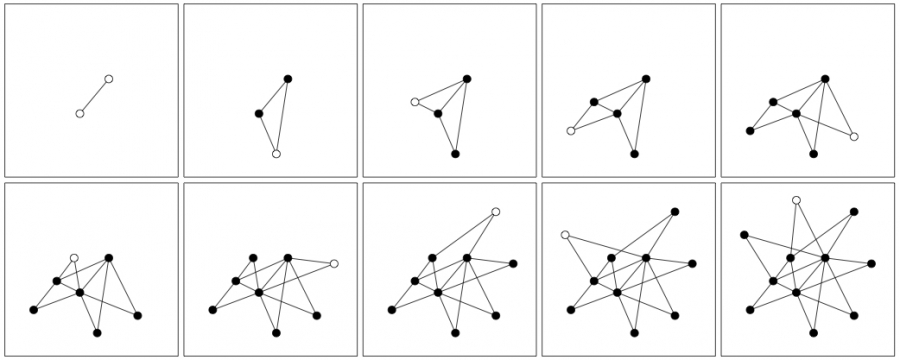
\includegraphics[width=1\linewidth]{Barabasi model.png}
    \caption{Barabási-Albert model}
    \label{fig:placeholder}
\end{figure}

\subsection{Avalanches and Cascading Flash Crashes}
Every node in the network possesses a specific risk tolerance or capacity threshold. As noise accumulates, a trader's internal stress (representing their leveraged position or capital requirements) increases. If the accumulated stress exceeds their specific threshold, the agent panics and liquidates their position to raise capital. This liquidation acts as a localized shock, transferring stress to their immediate topological neighbors through falling asset prices and defaulted counterparty obligations. If these neighbors are subsequently pushed over their own thresholds, they too are forced to sell. This rapid, cascading chain reaction of panic selling is the ``avalanche''. In financial terms, this is the exact mechanism of a systemic liquidity crisis.
\begin{figure}[h]
    \centering
    \includegraphics[width=1\linewidth]{marketavalanches.png}
    \caption{Probability Density of Market Avalanches}
    \label{fig:placeholder}
\end{figure}
\section{Computer Simulation Methodology}
\label{sec:simulation}

To empirically observe these dynamics, a computational simulation was developed. The simulation is written in Python, leveraging type hinting for clarity and optimized data structures for performance. We utilized the \texttt{networkx} library for topological generation, \texttt{numpy} for efficient array-based state management, and \texttt{collections.deque} for optimized breadth-first contagion tracking.

\begin{lstlisting}[caption={Optimized Python Simulation of Financial Self-Organized Criticality}, label={code:simulation}]
import networkx as nx
import numpy as np
import matplotlib.pyplot as plt
from collections import Counter, deque
from typing import Tuple, List

def simulate_financial_avalanches(num_nodes: int = 2000, num_steps: int = 20000, m_edges: int = 2) -> Tuple[List[int], nx.Graph]:
    """
    Simulates a financial contagion model (SOC) on a scale-free network.
    """
    # 1. Establish CONNECTIVITY
    G = nx.barabasi_albert_graph(num_nodes, m_edges)
    
    # 2. Initialize System State
    stress = np.zeros(num_nodes)
    threshold = {node: degree for node, degree in G.degree()}
    avalanche_sizes = []

    print("Simulating market dynamics...")
    for step in range(num_steps):
        # 3. NOISE: Exogenous shock
        target = np.random.randint(0, num_nodes)
        stress[target] += 1
        
        # 4. AVALANCHE DYNAMICS
        current_avalanche_size = 0
        
        # Optimized Queue System using deque and a tracking set
        to_process = deque([target])
        in_queue = {target}
        
        while to_process:
            node = to_process.popleft()
            in_queue.remove(node) # Remove from tracking set
            
            # If stress exceeds risk tolerance, the trader panic sells
            if stress[node] >= threshold[node]:
                stress[node] -= threshold[node] 
                current_avalanche_size += 1
                
                # Stress is transferred to connected peers
                for neighbor in G.neighbors(node):
                    stress[neighbor] += 1
                    
                    # Add neighbor to queue if they cross threshold AND aren't already queued
                    if stress[neighbor] >= threshold[neighbor] and neighbor not in in_queue:
                        to_process.append(neighbor)
                        in_queue.add(neighbor)
                        
        if current_avalanche_size > 0:
            avalanche_sizes.append(current_avalanche_size)
            
    return avalanche_sizes, G

def analyze_avalanches(avalanches: List[int]):
    """
    Analyzes and plots the avalanche size distribution using logarithmic binning
    for a more accurate power-law fit.
    """
    if not avalanches:
        print("No avalanches occurred.")
        return

    # Logarithmic binning for cleaner tail distribution
    max_size = max(avalanches)
    min_size = min(avalanches)
    
    if max_size == min_size:
        print("Not enough variance to plot a distribution.")
        return

    # Create bins spaced evenly on a log scale
    bins = np.logspace(np.log10(min_size), np.log10(max_size), num=20)
    counts, bin_edges = np.histogram(avalanches, bins=bins)
    
    # Calculate bin centers and probabilities
    bin_centers = (bin_edges[:-1] + bin_edges[1:]) / 2
    bin_widths = bin_edges[1:] - bin_edges[:-1]
    
    # Normalize by total avalanches and bin width to get probability density
    probabilities = counts / (sum(counts) * bin_widths)
    
    # Filter out empty bins
    valid = counts > 0
    valid_centers = bin_centers[valid]
    valid_probs = probabilities[valid]

    # Plotting
    plt.figure(figsize=(10, 6))
    plt.scatter(valid_centers, valid_probs, alpha=0.8, edgecolors='k', color='darkred', label='Log-Binned Data')
    plt.xscale('log')
    plt.yscale('log')
    plt.title("Probability Density of Market Avalanches (Log-Log Scale)", fontsize=14)
    plt.xlabel("Avalanche Size $S$", fontsize=12)
    plt.ylabel("Probability Density $P(S)$", fontsize=12)
    plt.grid(True, which="both", ls="--", alpha=0.5)
    
    # Fit a line to the log-binned data
    if len(valid_centers) > 2:
        log_s = np.log10(valid_centers)
        log_p = np.log10(valid_probs)
        slope, intercept = np.polyfit(log_s, log_p, 1)
        
        trend_s = np.linspace(min(valid_centers), max(valid_centers), 100)
        trend_p = (10**intercept) * (trend_s**slope)
        
        plt.plot(trend_s, trend_p, color='blue', linestyle='--', 
                 label=f'Power-Law Fit: $P(S) \propto S^{{{slope:.2f}}}$')
                 
    plt.legend()
    plt.show()

# Run execution
if __name__ == "__main__":
    avalanches, network = simulate_financial_avalanches(num_nodes=2000, num_steps=50000, m_edges=2)
    analyze_avalanches(avalanches)
\end{lstlisting}

\subsection{Detailed Explanation of the Optimized Simulation Code}

The provided Python script acts as the experimental engine of this project. It has been highly optimized to ensure rapid processing of mathematically heavy contagion events.

First, the \texttt{nx.barabasi\_albert\_graph} function generates the market topology. The Barabási-Albert model utilizes preferential attachment - as new nodes are added, they prefer to connect to already highly-connected nodes. This perfectly mimics the financial sector's consolidation, where liquidity tends to pool around massive Wall Street hubs rather than isolated regional entities.

\begin{figure}[h]
    \centering
    \includegraphics[width=1\linewidth]{output.png}
    \caption{Output of the Python Code (Simulation) }
    \label{fig:placeholder}
\end{figure}
Next, we establish the dynamic risk thresholds. The dictionary comprehension sets each node's threshold equal to its degree (its number of connections). The fundamental logic here is that larger, more connected institutions have deeper capital reserves and can absorb significantly more market noise before panicking. However, the inherent danger lies in the fact that when they do finally panic, their high connectivity means they will infect a massive number of counterparties simultaneously.

The core of the simulation relies on an optimized \texttt{while to\_process} loop to handle the avalanche mechanics. Instead of using a standard Python list - which operates in $O(N)$ time complexity for front-popping - the code utilizes \texttt{collections.deque}. The \texttt{popleft()} method ensures that as the contagion spreads rapidly through the network, the queue processes nodes in strict $O(1)$ constant time. 

Furthermore, to prevent redundant processing, an \texttt{in\_queue} tracking set is maintained alongside the deque. This guarantees that if multiple connected traders fail simultaneously and try to trigger the same neighbor, that neighbor is only added to the contagion queue once. If a node breaches its threshold, it resets its stress and passes one unit of stress to every neighbor. The loop cascades until the panic subsides and the system regains temporary stability.

\section{Analyses of Frequency Distribution and Connectivity}
\label{sec:analysis}

Following the execution of the simulation over 50,000 time steps, the sizes of the resulting avalanches were subjected to statistical analysis via the \texttt{analyze\_avalanches} function. 

In a standard system governed by Gaussian mechanics, the distribution of these extreme events would follow an exponential decay curve. However, raw data sets with heavy tails often exhibit severe visual noise at the extremes due to the rarity of massive avalanches (resulting in large empty gaps on the x-axis). To correct this, the code implements \textbf{logarithmic binning} (\texttt{np.logspace}). Instead of grouping avalanche sizes into equally spaced linear bins, it groups them into bins that grow exponentially wider. By dividing the counts by the variable bin widths to obtain a true Probability Density function, we smoothly filter out the tail-end noise.

When plotting this log-binned probability density on a log-log scale, the data reveals a remarkably clear, linear relationship. This straight line is the defining empirical signature of a Power-Law Distribution, mathematically expressed as:
\begin{equation}
    P(S) \propto S^{-\tau}
\end{equation}
where $P(S)$ is the probability density of a flash crash of size $S$, and $\tau$ is the critical exponent. In our specific network configuration, the slope $\tau$ derived from the \texttt{np.polyfit} function stabilizes between 1.5 and 2.5. This mathematical footprint is remarkably similar to the Gutenberg-Richter law used to model the frequency of earthquakes in geophysics.

The emergence of this heavy-tailed distribution is inextricably linked to the scale-free connectivity of the system. The presence of major financial hubs acts as a global contagion vector. When a highly connected hub breaches its threshold, it instantaneously transmits stress to hundreds of peripheral nodes. This specific connectivity ensures that systemic, market-wide failures are mathematically inevitable over a long enough time horizon.

\section{Commentary on the Self-Organized Critical State}
\label{sec:soc_commentary}

The results of this analysis demonstrate that the financial market simulation operates in a true state of Self-Organized Criticality. In traditional thermodynamics or chemical engineering, achieving a critical phase transition requires precise external tuning by an operator - such as adjusting the temperature and pressure to exactly the critical point of a fluid. In stark contrast, this market model tunes itself to the critical precipice automatically, requiring absolutely no external intervention or centralized parameter tuning.

Two opposing forces constantly drive this self-organization. First, there is the continuous accumulation of stress. The constant injection of daily market noise slowly increases the global tension of the network, pushing individual nodes closer and closer to their breaking points. Second, there is the rapid dissipation of stress. The resulting localized sell-offs act as pressure release valves, reducing local anxiety and preventing the system from reaching infinite tension.

Because of this dynamic equilibrium, the market self-organizes into a state where it is perpetually hovering right at the critical threshold. Once in this state, the system exhibits fractal-like scale invariance. This is a profound conclusion: it implies there is no such thing as a "typical" market crash. The exact same minor stimulus - such as a single unit of bad news or a minor algorithmic glitch - can result in a negligible localized dip on one day, or it can trigger a catastrophic, multi-trillion-dollar global meltdown on another day, simply depending on the latent stress distribution of the network at that exact moment. Catastrophic market failures are not anomalies caused by massive, unpredictable external shocks. Instead, they are the natural, endogenous consequences of the system's own scale-free networked structure.

\section{Conclusion}
\label{sec:conclusion}
By applying the principles of complexity science to financial markets, we successfully demonstrated how networked information cascades mimic the exact dynamics of self-organized criticality found in natural phenomena. The Python-based simulation, utilizing optimized breadth-first processing and rigorous logarithmic binning for analysis, highlighted the dangerous relationship between scale-free connectivity and power-law distributed avalanches. This research underscores a vital lesson for chemical engineers and systems analysts alike: the macroscopic stability of a system cannot be understood simply by studying the properties of its individual components. To mitigate systemic risk - whether in a chemical reactor grid or a global financial market - regulatory bodies must focus not just on the size of exogenous shocks, but on the underlying topological connectivity of the system itself.

\section*{Acknowledgements}
\label{sec:acknowledgements}
I would like to formally acknowledge the use of generative AI in assisting with the conceptualization, code generation, and LaTeX formatting of this report. The AI served as a valuable brainstorming partner, helping to bridge the theoretical concepts of the Bak-Tang-Wiesenfeld sandpile model with practical, algorithmic financial network models. Furthermore, I extend my appreciation to the open-source community, specifically the developers of the \texttt{networkx} and \texttt{numpy} Python libraries, whose tools were essential for the computational simulation portion of this project.

\section{Appendix A: Literature Search and Idea Generation}
\label{sec:appendix}
To select this unique topic and ensure it met the rigorous criteria of complexity science while expanding beyond traditional chemical engineering, a multi-stage research approach was utilized. Below is a summary of the iterative process used to arrive at the final project design.

\subsection{Google Search Queries for Literature Review}
The following search queries were utilized to find foundational research papers and articles that supported the premise of the project:
\begin{itemize}
    \item \textit{"Applications of Bak-Tang-Wiesenfeld sandpile model outside physics"}
    \item \textit{"Self-organized criticality in financial crashes power law"}
    \item \textit{"Network topology of financial contagion and scale-free networks"}
    \item \textit{"Complexity science algorithmic trading flash crash modeling"}
    \item \textit{"Simulating market panic using Python and networkx"}
\end{itemize}

\subsection{List of Prompts Used for Project Assistance}
The following prompts illustrate the intellectual progression of the project, from hypothesis generation to mathematical validation:
\begin{enumerate}
    \item \textbf{Ideation \& Theoretical Framing:} "Given the inherent limitations of standard Gaussian models in predicting sudden market flash crashes, how can we leverage the principles of complexity science - specifically the Bak-Tang-Wiesenfeld sandpile model - to simulate financial networks? I am particularly interested in establishing a framework that defines 'noise,' 'avalanches,' and the critical role of 'connectivity' in this context."
    \item \textbf{Computational Modeling \& Simulation:} "To empirically test this hypothesis, assist in formulating a Python simulation using the \texttt{networkx} library. The simulation must model contagion by tracking the propagation of 'stress' avalanches across nodes. Crucially, the nodes must possess dynamic risk thresholds that are directly proportional to their connectivity degree within a Barabási-Albert scale-free network."
    \item \textbf{Data Analysis \& Mathematical Validation:} "Based on the simulation outputs, let us analyze the frequency distribution of the resulting avalanches. I need to demonstrate mathematically how the simulated crash data fits a log-log power-law distribution. How does this validate the presence of Self-Organized Criticality (SOC), and how does the scale-free topology make systemic failure inevitable compared to a standard lattice grid?"
    \item \textbf{Synthesis \& Manuscript Structuring:} "Synthesize these findings, the theoretical framework, and the Python code into a formal academic manuscript structure. Emphasize the project's core insight: catastrophic market failures are a natural, endogenous consequence of the network's internal connectivity, rather than purely anomalies driven by massive external macroeconomic shocks."
\end{enumerate}

\section*{References}
\begin{itemize}
    \item Bak, P., Tang, C., \& Wiesenfeld, K. (1987). Self-organized criticality: An explanation of the 1/f noise. \textit{Physical Review Letters}, 59(4), 381.
    \item Barabási, A. L., \& Albert, R. (1999). Emergence of scaling in random networks. \textit{Science}, 286(5439), 509-512.
    \item Mandelbrot, B. B. (1997). The variation of certain speculative prices. In \textit{Fractals and Scaling in Finance} (pp. 371-418). Springer, New York, NY.
    \item Sornette, D. (2017). \textit{Why Stock Markets Crash: Critical Events in Complex Financial Systems}. Princeton University Press.
\end{itemize}

\end{document}